\documentclass[a4paper]{article}
\usepackage{graphicx} % Required for inserting images
\usepackage{tikz}
\usepackage[margin=1cm]{geometry}

% Adapted from A-maze-ing on emaths.co.uk
% initial version of diagram created by claude.ai in response to prompt:
% I would like a TikZ artefact. I want the diagram to be a 4x4 grid of circles, with bold mathematical operators within them, such as 'x9' and '+3'.


\title{\vspace{-1.5cm}A---maze---ing - Year 1}
\author{Jarvist Moore Frost}
\date{8th September 2024}

\begin{document}


\maketitle

In the maze, travel from START to END moving only right or down. 

 - START with Zero (0), can you find a route which makes 10 at the END?

 - What is the biggest number you can make?

 - How many different routes are there through the maze?

\vspace{1.0cm}

\centering

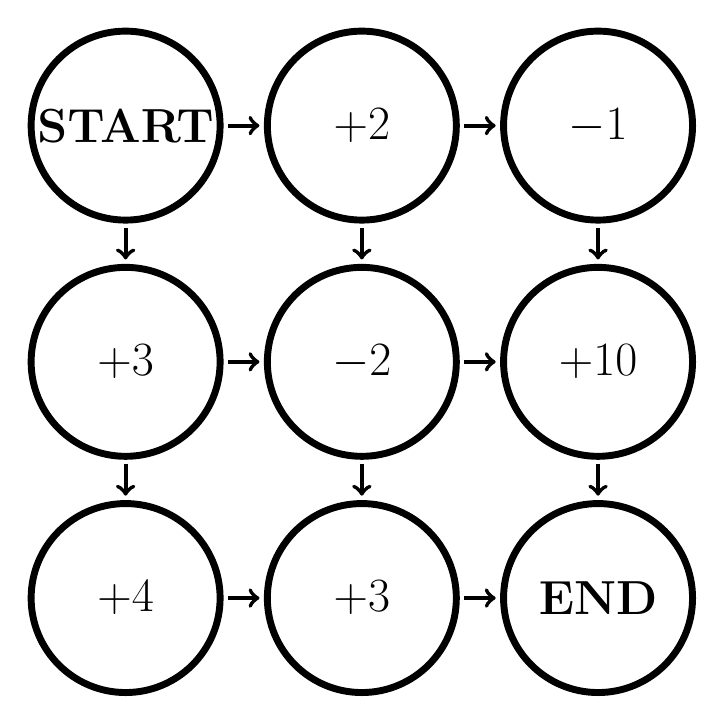
\begin{tikzpicture}[font=\bfseries\Large]
  % Draw circles and arrows
  \foreach \x in {0,...,2} {
    \foreach \y in {0,...,2} {
      \draw[line width=2.5pt] (\x*3,\y*3) circle (1.2cm);
      
      % Draw right arrow if not in the last column
      \ifnum\x<2
        \draw[->, line width=1.5pt] (\x*3+1.3,\y*3) -- (\x*3+1.7,\y*3);
      \fi
      
      % Draw down arrow if not in the last row (corrected condition)
      \ifnum\y<2
        \draw[->, line width=1.5pt] (\x*3,\y*3+1.7) -- (\x*3,\y*3+1.3);
      \fi
    }
  }
  
  % Fill in the circles with larger operators
  \node[font=\bfseries\LARGE] at (0,6) {START};
  \node[font=\bfseries\LARGE] at (3,6) {$+2$};
  \node[font=\bfseries\LARGE] at (6,6) {$-1$};
  
  \node[font=\bfseries\LARGE] at (0,3) {$+3$};
  \node[font=\bfseries\LARGE] at (3,3) {$-2$};
  \node[font=\bfseries\LARGE] at (6,3) {$+10$};
  
  \node[font=\bfseries\LARGE] at (0,0) {$+4$};
  \node[font=\bfseries\LARGE] at (3,0) {$+3$};
  \node[font=\bfseries\LARGE] at (6,0) {END};
\end{tikzpicture}

\vspace{1.0cm}

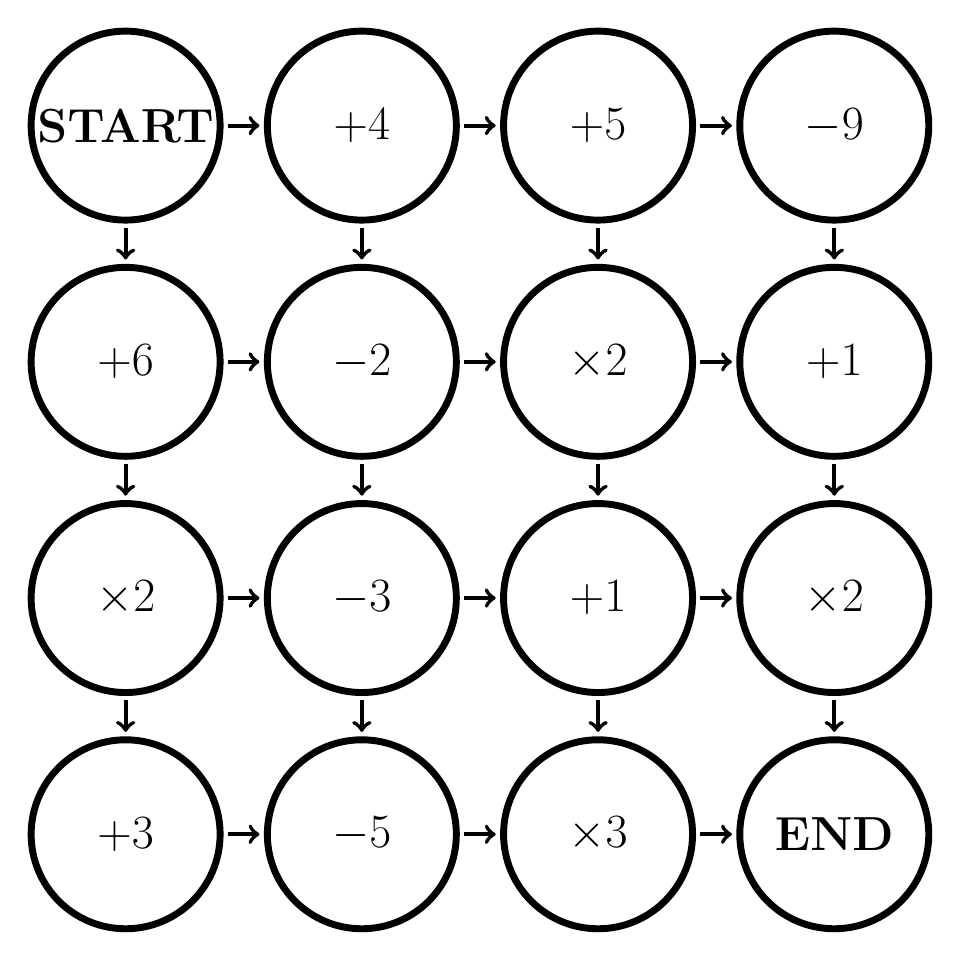
\begin{tikzpicture}[font=\bfseries\Large]
  % Draw circles and arrows
  \foreach \x in {0,...,3} {
    \foreach \y in {0,...,3} {
      \draw[line width=2.5pt] (\x*3,\y*3) circle (1.2cm);
      
      % Draw right arrow if not in the last column
      \ifnum\x<3
        \draw[->, line width=1.5pt] (\x*3+1.3,\y*3) -- (\x*3+1.7,\y*3);
      \fi
      
      % Draw down arrow if not in the last row (corrected condition)
      \ifnum\y<3
        \draw[->, line width=1.5pt] (\x*3,\y*3+1.7) -- (\x*3,\y*3+1.3);
      \fi
    }
  }
  
  % Fill in the circles with larger operators
  \node[font=\bfseries\LARGE] at (0,9) {START};
  \node[font=\bfseries\LARGE] at (3,9) {$+4$};
  \node[font=\bfseries\LARGE] at (6,9) {$+5$};
  \node[font=\bfseries\LARGE] at (9,9) {$-9$};
  
  \node[font=\bfseries\LARGE] at (0,6) {$+6$};
  \node[font=\bfseries\LARGE] at (3,6) {$-2$};
  \node[font=\bfseries\LARGE] at (6,6) {$\times2$};
  \node[font=\bfseries\LARGE] at (9,6) {$+1$};
  
  \node[font=\bfseries\LARGE] at (0,3) {$\times2$};
  \node[font=\bfseries\LARGE] at (3,3) {$-3$};
  \node[font=\bfseries\LARGE] at (6,3) {$+1$};
  \node[font=\bfseries\LARGE] at (9,3) {$\times2$};
  
  \node[font=\bfseries\LARGE] at (0,0) {$+3$};
  \node[font=\bfseries\LARGE] at (3,0) {$-5$};
  \node[font=\bfseries\LARGE] at (6,0) {$\times3$};
  \node[font=\bfseries\LARGE] at (9,0) {END};
\end{tikzpicture}
\end{figure}



\end{document}
